\documentclass[10 pt]{article}
\usepackage{tikz}
\usetikzlibrary{arrows}
\usepackage[margin=0.5 in]{geometry}
\usepackage[utf8]{inputenc}
\usepackage{tabu}
\usepackage{color}
\usepackage{mathtools}
\usepackage{amsfonts}
\usepackage{xcolor}
\usepackage{listings}
\usepackage{enumitem}
\usepackage{multicol}
\setlength{\columnsep}{1cm} 
\newtheorem{theorem}{Teorema}
\usepackage{mathrsfs}
\title{\textbf {Estructuras de Datos y Algoritmos 1 - ST0245\\Segundo Parcial 001 - Jueves}}
\author{Nombre ..............................\\
		Departamento de Informática y Sistemas\\
		Universidad EAFIT\\}
\date{Mayo 13 de 2021}
\begin{document}

\lstset{language=Java,frame=none, breaklines=true, numbers = left, stepnumber = 1, xleftmargin=5.0ex, showstringspaces=false, showspaces=false }
\lstset{language=Python,frame=none, breaklines=true, numbers = left, stepnumber = 1, xleftmargin=5.0ex, showstringspaces=false,showspaces=false }
\maketitle

\section{Árboles 30\%}
En la vida real, los árboles binarios de búsqueda (BST) se usan en bases de datos relacionales como MySQL de Oracle, SQL Server de Microsoft o DB2 de IBM. 
¿Te gustaría trabajar en una de estas empresas? Bueno, vamos a resolver un problema con BSTs. 
 Dado un conjunto de números $a$, donde $a_i \leq a_j \iff i < j$, crea un BST con el conjunto de números $a$. Si estás muy emocionado con bases de datos, imagina que $a$ son las llaves primarias de una tabla. Si hay múltiples respuestas, cualquiera de ellas es válida. Para el conjunto de números $a = [1, 2, 3, 4, 5, 6, 7 , 8, 9, 10]$, la respuesta es la siguiente:
\begin{center}
    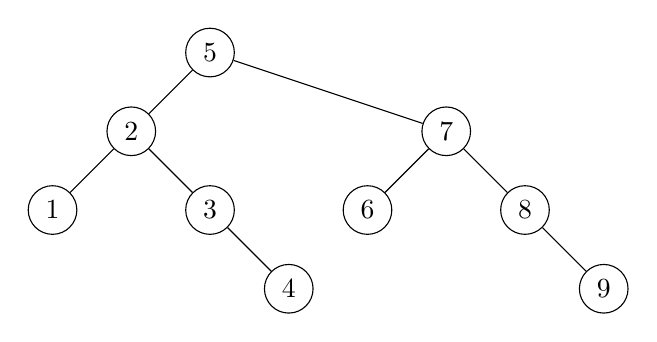
\begin{tikzpicture}
    
    \tikzset{vertex/.style = {shape=circle,draw,minimum size=1.5em}}
    \tikzset{edge/.style = {-,> = latex'}}
    \node[vertex] (G) at (0,0)  {5};
    \node[vertex] (I) at (3,-1)  {7};
    \node[vertex] (H) at (2,-2)  {6};
    \node[vertex] (J) at (4,-2)  {8};
    \node[vertex] (D) at (-1, -1) {2};
    \node[vertex] (E) at (0, -2) {3};
    \node[vertex] (F) at (1, -3) {4};
    \node[vertex] (B) at (-2, -2) {1};
    \node[vertex] (A) at (5, -3) {9};
    %edges
    \draw[edge] (G) to (D);
    \draw[edge] (D) to (B);
    \draw[edge] (D) to (E);
    \draw[edge] (E) to (F);
    \draw[edge] (G) to (I);
    \draw[edge] (I) to (H);
    \draw[edge] (I) to (J);
    \draw[edge] (A) to (J);
    \end{tikzpicture}
  \end{center}

La respuesta a este problema está en el siguiente algoritmo, pero faltan algunas líneas.

\hspace{1 cm}

\textbf{Si trabajas en Java}, considera el siguiente código:

\begin{lstlisting}[language=java]
class Node {
  int data;
  Node left;
  Node right
  Node(int d){data = d;}
}
private Node solve(int[] a, int l, int r) {
  if (l > r) {
    return null;
  }
  int m = l + (r - l) / 2;
  Node root = new Node(a[m]);
  root.left = ........................;
  root.right = .......................;
  return root;
}
public Node solve(int[] a){
  return solve(a, 0, a.length - 1);
}
\end{lstlisting}

\begin{enumerate}[label=(\Alph*)]
% Respuesta: solve(a, l, m - 1) en Java o solveAux(a, l, m - 1) en Python
\item (10\%) Completa la línea 13 .......................
% Respuesta: solve(a, m + 1, r) en Java o solveAux(a, l, m - 1) en Python
\item (10\%) Completa la línea 14 .......................
% T(n) = 2*T(n/2) + c, que es O(n)
\item (10\%) ¿Cuál es la ecuación de recurrencia para el peor de los casos? \\
T(n) = ................. donde $n$ es el número de elementos de $a$

\end{enumerate}

\newpage

\textbf{Si trabajas en Python}, considera el siguiente código:

\begin{lstlisting}[language=python]
class Node:
  def __init__(self,d):
    self.data = d
    self.left = None
    self.right = None

def solveAux(a, l, r):
  if l > r:
    return None
  
  m = int(l + (r - l) / 2)
  root = Node(a[m])
  root.left = ........................
  root.right = .......................
  return root

def solve(a):
  return solveAux(a, 0, len(a) - 1)
\end{lstlisting}

\begin{enumerate}[label=(\Alph*)]
% Respuesta: solve(a, l, m - 1) en Java o solveAux(a, l, m - 1) en Python
\item (10\%) Completa la línea 13 .......................
% Respuesta: solve(a, m + 1, r) en Java o solveAux(a, l, m - 1) en Python
\item (10\%) Completa la línea 14 .......................
% T(n) = 2*T(n/2) + c, que es O(n)
\item (10\%) ¿Cuál es la ecuación de recurrencia para el peor de los casos? \\
T(n) = ................. donde $n$ es el número de elementos de $a$
\end{enumerate}

\begin{center}
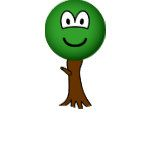
\includegraphics[width=0.3\textwidth]{tree.jpg}
\end{center}

\newpage



\section{Pilas 20\%}


La \textit{Notación polaca inversa} es una notación matemática en la cual los operadores siguen sus operandos. En la vida real, la notación polaca inversa fue ampliamente utilizada, en los años 70s y 80s, por las calculadoras científicas 
Hewlett-Packaar. Por ejemplo, la expresión en notación polaca $5\;31\;4 + \times$, equivale a la expresión $(31 + 4) \times 5$. Dado  un arreglo de operadores y operandos (\textit{tokens}) que representan una expresión en notación polaca, considerando sólo  los operadores ``(+, *, -, /)'', determina el resultado de la expresión. Utilizando una pila, es posible operar una expresión en esta notación, así:

\hspace{1 cm}

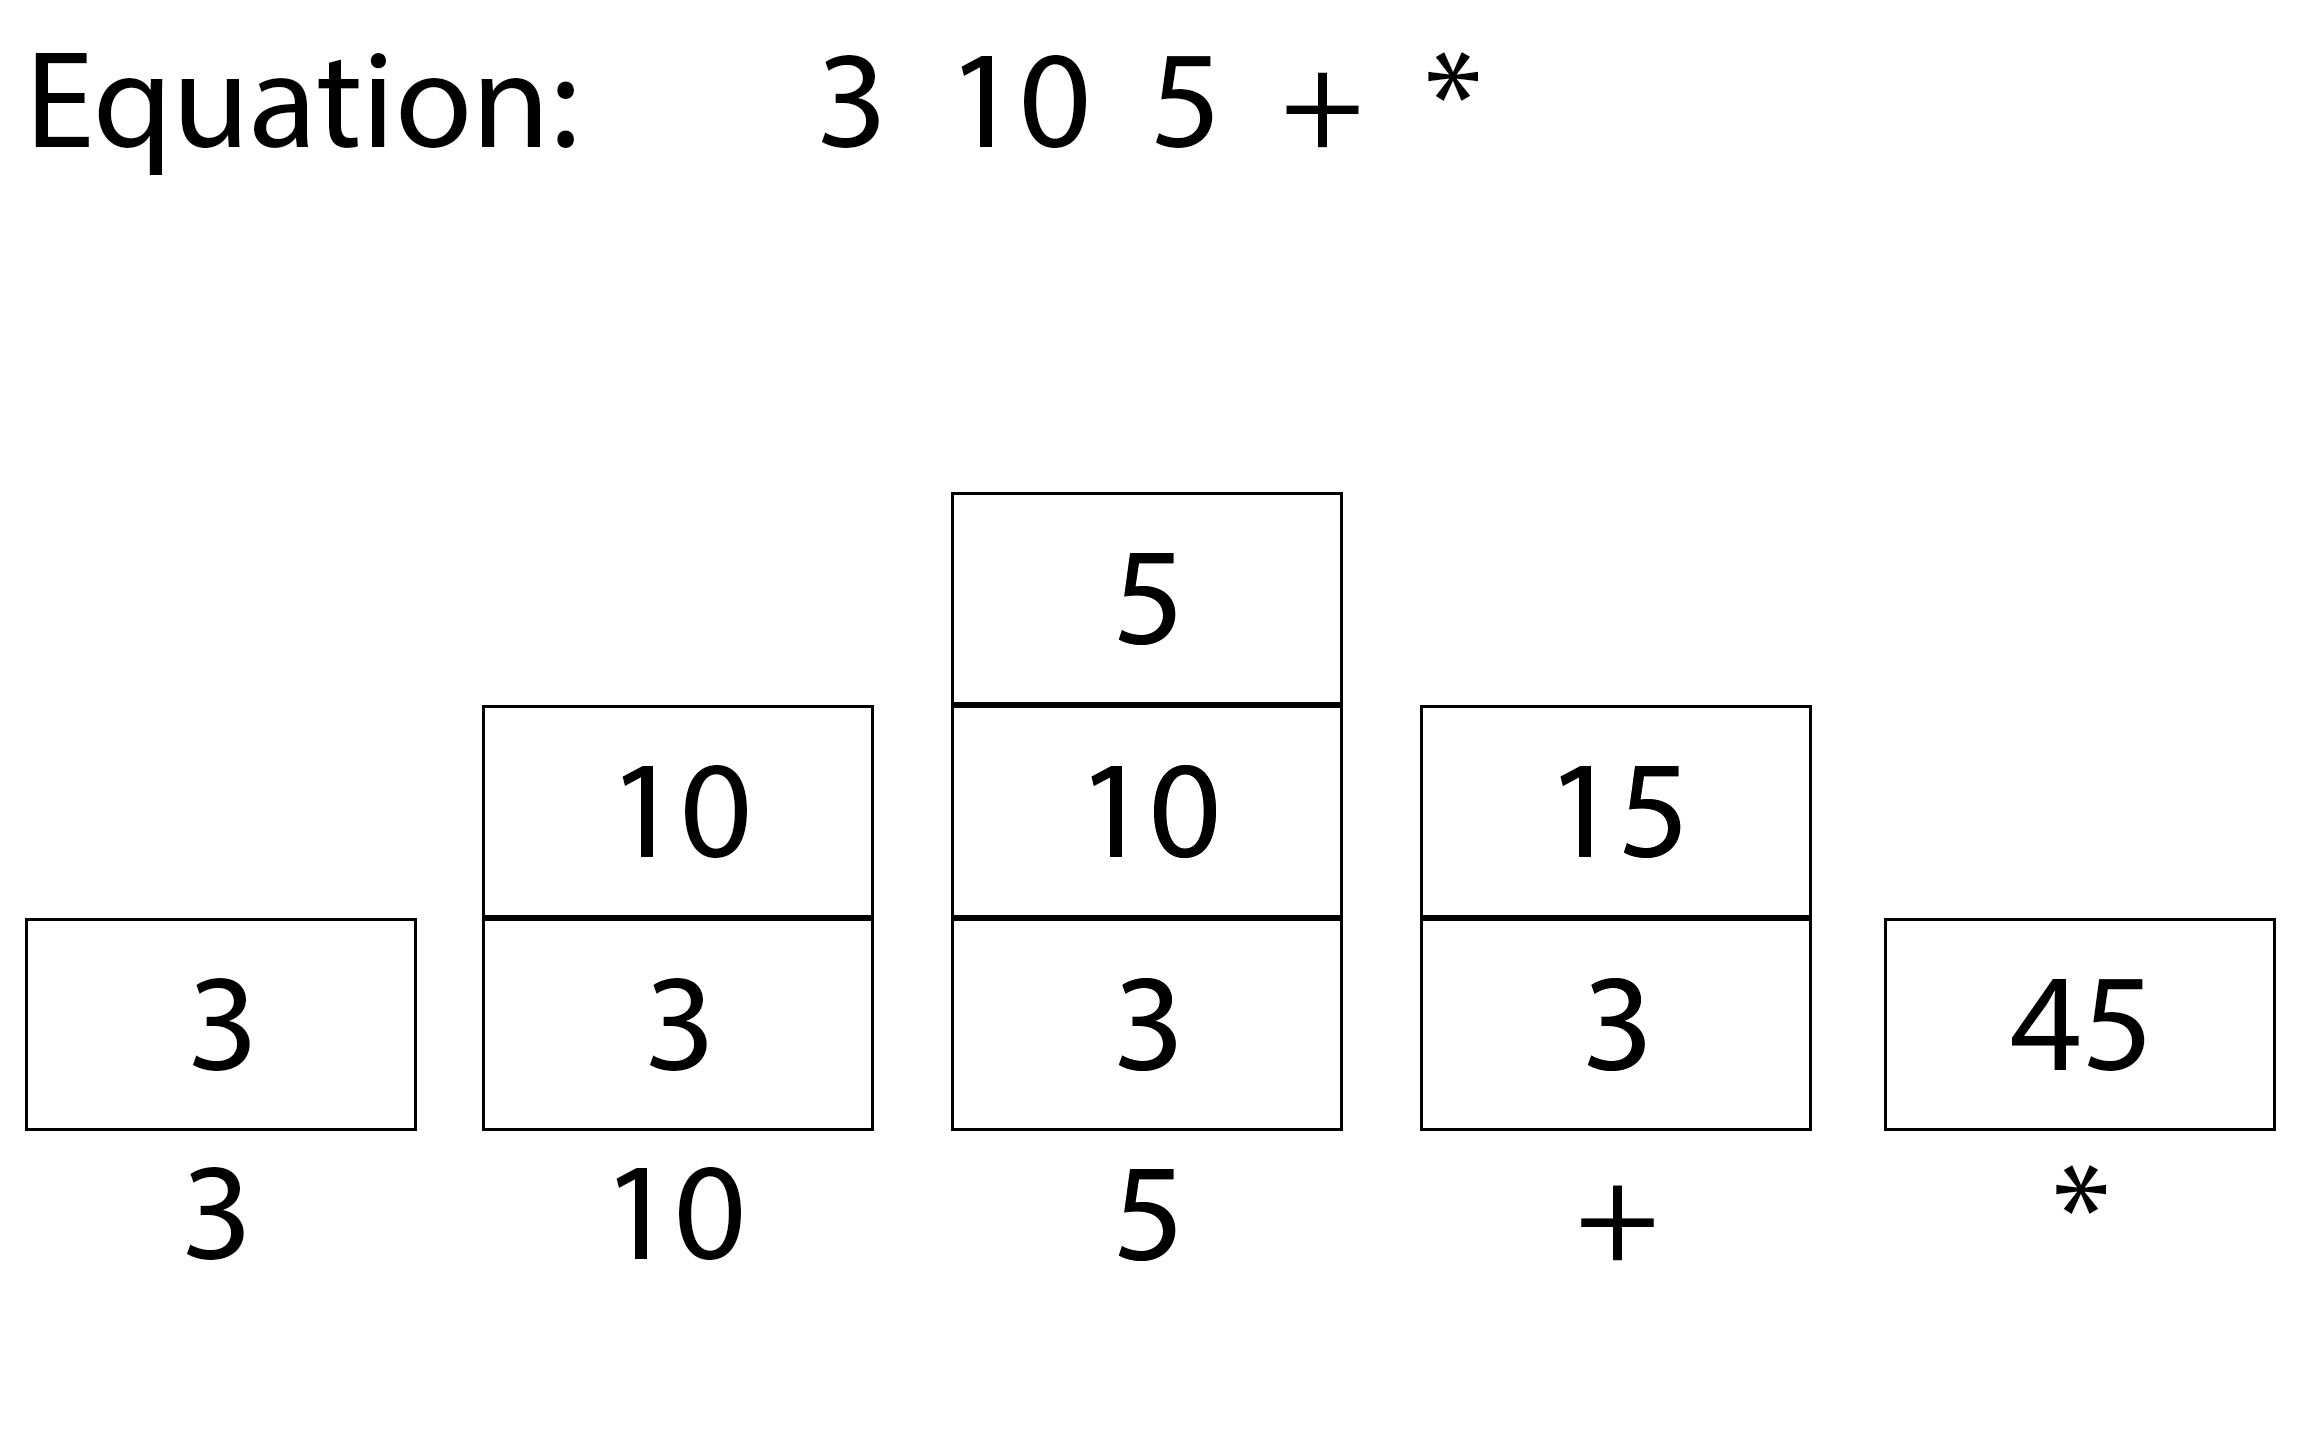
\includegraphics[scale=0.07]{ReversePolishNotationStackExample.jpg}


Ya hemos adelantado algo de trabajo, pero falta completar algunas líneas, por favor.

\hspace{1 cm}

\textbf{Si trabajas en Java}, considera el siguiente código:

\begin{lstlisting}[language = Java]
int solve(String[] tokens){
  String operators = "+-*/";
  Stack<String> aStack = new Stack<String>();
  for(String t : tokens){
    if(!operators.contains(t)){
      ..............;
    }else{
      int a = ..................;
      int b = ..................;
      int index = operators.indexOf(t);
      if(index == 0) 
       aStack.push(String.valueOf(a+b));
      else if(index == 1)
       aStack.push(String.valueOf(b-a));
      else if(index == 2)
       aStack.push(String.valueOf(a*b));
      else // index == 3
       aStack.push(String.valueOf(b/a));
    }
  }
  return ...............;
}
\end{lstlisting}
\begin{enumerate}[label=(\Alph*)]
 
  % Solución Java: aStack.push(t)
  \item (10\%) Completa la línea 6\\
  \line(1, 0){230}\\
  % Solución Java: Integer.valueOf(aStack.pop()),Integer.valueOf(aStack.pop())
  \item (10\%) Completa las líneas 8 y 9\\
  \line(1, 0){230} \\
  \line(1, 0){230}\\
  % Solución Java: Integer.valueOf(aStack.pop())
  Y completa la línea 21\\
  \line(1, 0){230}
\end{enumerate}

En Java, el método \texttt{String.valueOf(a)} convierte el entero $a$ en una cadena de caracteres y el método \texttt{Integer.valueOf(b)} convierte la cadena $b$ en un entero.

\newpage

\textbf{Si trabajas en Python}, considera el siguiente código:

\begin{lstlisting}[language = Python]
def solve(tokens):
  operators = "+-*/"
  aStack = deque()
  for t in tokens:
    if not t in operators:
      ..................
    else:
      a = .........
      b = ..........
      index = operators.index(t)
      if index == 0:
       aStack.append(str(a+b))
      elif index == 1:
       aStack.append(str(a-b))
      elif index == 2:
       aStack.append(str(a*b))
      else: #index == 3
       aStack.append(str(b/a))
  return ...............
\end{lstlisting}

\begin{enumerate}[label=(\Alph*)]
 
  % Solución Python: aStack.append(t)
  \item (10\%) Completa la línea 6\\
  \line(1, 0){230}\\
  % Solución Python: int(aStack.pop())   y   int(aStack.pop())
  \item (10\%) Completa las líneas 8 y 9\\
  \line(1, 0){230} \\
  \line(1, 0){230}\\
  % Solución Python: int(aStack.pop())
  Y completa la línea 19\\
  \line(1, 0){230}
\end{enumerate}

En Python, la librería \texttt{deque} se usa para implementar una pila. 
En \texttt{deque}, \texttt{append()} agrega al final y \texttt{pop()} elimina el elemento del final. 
Además, en Python, la función \texttt{str(a)} convierte el entero $a$ en una cadena de caracteres y la función \texttt{int(b)} convierte la cadena $b$ en un entero.


\begin{center}
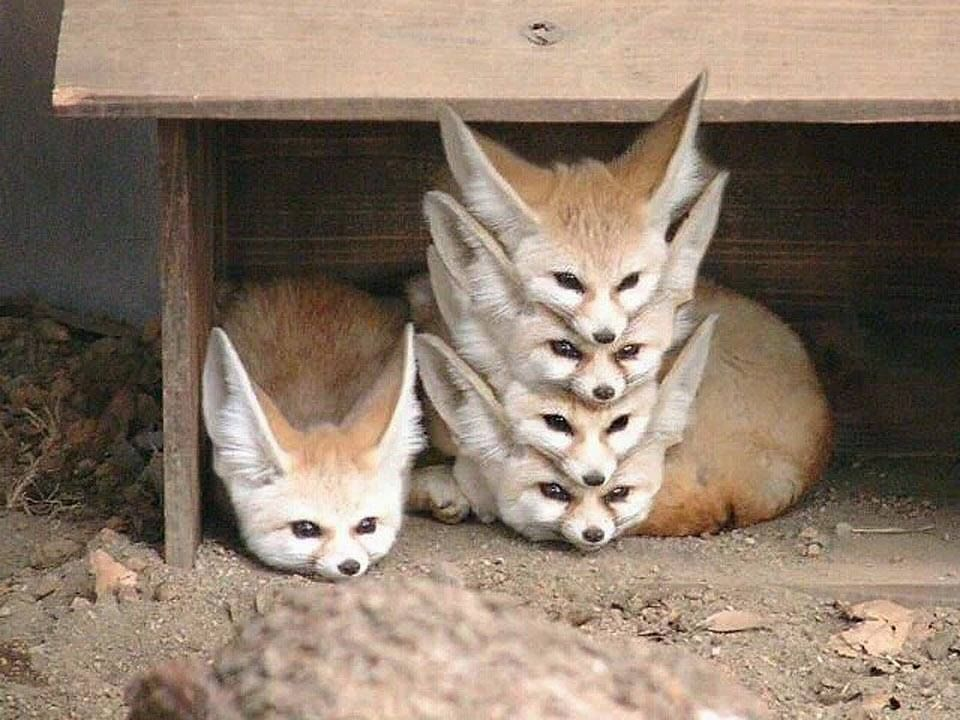
\includegraphics[width=0.3\textwidth]{stack.jpg}
\end{center}

\newpage





\section{Colas 20\%}


En la vida real,  hacemos filas de espera (\textit{Queues}) para entrar a un parqueadero, para ser atendido en un banco o para comprar un producto en un supermercado.
 Implementar filas de espera, en un programa informático, es importante para simular, por ejemplo, el impacto que tendría
 --sobre los tiempos de espera-- el contratar un nuevo cajero. Por eso, estas implementaciones son de suma importancia para empresas como Bancolombia. 
La siguiente clase implementa una fila de espera para un máximo de $n$ elementos. Tan sólo hace falta calcular la complejidad asintótica, para el peor de los
casos, de las operaciones entrar a la fila de esperar (\textit{enqueue}) y salir de la fila de espera (\textit{dequeue}). 

\hspace{1 cm}

\textbf{Si trabajas en Java}, considera el siguiente código:

\begin{lstlisting}[language = Java]
class Queue {
  int e[];
  int index;
  boolean started;

  Queue(int n) {
    e = new int[n];
    index = 0;
    started = false;
  }

  public boolean isEmpty() {
    return (index == 0 && !started) | index <= 0;
  }

  void enqueue(int x){
    if (index == e.length) {
      throw new RuntimeException("Full");
    }
    started = true;
    e[index] = x;
    index++;
  }

  int dequeue(){
    if (isEmpty())
      throw new RuntimeException("Empty");
    int x = e[0];
    for (int i = 0; i < index - 1; i++) {
      e[i] = e[i + 1];
    }
    index--;
    return x;
  }
}
\end{lstlisting}

\begin{enumerate}[label=(\Alph*)]
  % O(1)
  \item (10\%) Calcula la complejidad asintótica, para el peor de los casos, de 
   \texttt{enqueue(x)} \\ \\
   O(\line(1, 0){230})\\

  % O(n)
  \item (10\%) Calcula la complejidad asintótica, para el peor de los casos, de 
   \texttt{dequeue(x)} \\ \\
   O(\line(1, 0){230})\\


\end{enumerate}

\newpage

\textbf{Si trabajas en Python}, considera el siguiente código:

\begin{lstlisting}[language = Python]
import numpy as np
class Queue:

  def __init__(self, n):
    self.e = np.zeros(n)
    self.index = 0;
    self.started = False;

  def isEmpty(self): 
    return (self.index == 0 and not self.started) or self.index <= 0

  def enqueue(self,x):
    if self.index == self.e.size:
      raise Exception("Full")
    self.started = True
    self.e[self.index] = x
    self.index = self.index + 1

  def dequeue(self):
    if self.isEmpty():
      raise Exception("Empty")
    x = self.e[0]
    for i in range (0, self.index - 1):
      self.e[i] = self.e[i + 1]
    self.index = self.index - 1
    return x
\end{lstlisting}




\begin{enumerate}[label=(\Alph*)]

  \item (10\%) Calcula la complejidad asintótica, para el peor de los casos, de 
   \texttt{enqueue(x)} \\ \\
   O(\line(1, 0){230})\\

  \item (10\%) Calcula la complejidad asintótica, para el peor de los casos, de 
   \texttt{dequeue(x)} \\ \\
   O(\line(1, 0){230})\\


\end{enumerate}

\newpage



\section{Tablas de Hash 20\%}
En la vida real, el siguiente problema es frecuente en entrevistas para conseguir un trabajo en empresas como Microsoft, Google y Amazon, según
el portal \textit{Geeks for Geeks}. El problema es el siguiente. Dadas dos cadenas $S$ y $P$, encuentra la ventana más pequeña de $S$ formada por todos los caracteres de $P$. Tu tarea es completar la función \texttt{findSubString()} que toma dos cadenas $S$ y $P$ como parámetros de entrada y devuelve la ventana más pequeña de la cadena $S$ que tenga todos los caracteres de la cadena $P$. En caso de que haya varias ventanas de la misma longitud, devuelve la que tenga el menor índice inicial. Devuelve "-1" en caso de que no haya ninguna ventana de este tipo. A continuación, algunos ejemplos:

\begin{itemize}
  \item
\noindent
\textbf{Entrada:} S = "timetopráctica" y P = "toc"
\noindent
\textbf{Salida:} toprac
\noindent
\textbf{Explicación:} "toprac" es la subcadena más pequeña
subcadena en la que se puede encontrar "toc".
\item 
\noindent
\textbf{Entrada:} S = "zoomlazapzo" y P = "oza"
\noindent
\textbf{Salida:}  apzo
\noindent
\textbf{Explicación:} "apzo" es la subcadena más pequeña 
en la que se puede encontrar "oza".
\end{itemize}


\hspace{1 cm}

\textbf{Si trabajas en Java}, considera el siguiente código:

{\footnotesize
\begin{lstlisting}[language = java]
    static final int no_of_chars = 256;
    // Encontrar la ventana mas pequenha con los caracteres de pat
    static String findSubString(String str, String pat) {
        int len1 = str.length();
        int len2 = pat.length();
        // Mirar si la longitud de la cadena str es menor a la del patron pat
        if (len1 < len2) 
            return "-1";        
        int hash_pat[] = new int[no_of_chars];
        int hash_str[] = new int[no_of_chars];        
        // Guardar las ocurrencias de caracteres del patron pat
        for (int i = 0; i < len2; i++)
            hash_pat[pat.charAt(i)]++;
        int start = 0, start_index = -1,
            min_len = Integer.MAX_VALUE;   // MAX_VALUE es "infinito"
        int count = 0;
        for (......................) {
            // Contar las ocurrencias de los caracteres en la cadena 
            hash_str[str.charAt(j)]++;
            // Si los caracteres esta en el patron pat y cadena str, contar
            if (hash_str[str.charAt(j)] <= hash_pat[str.charAt(j)])
                count++; 
            // Si los caracteres de pat son tantos como el contador count 
            if (count == len2) {               
                // Intentar buscar una ventana mas pequenha
                while (....................................) { 
                    if (hash_str[str.charAt(start)] > hash_pat[str.charAt(start)])
                        hash_str[str.charAt(start)]--;
                    start++;
                }
                // Actualizar el tamanho de la ventana 
                int len_window = j - start + 1;
                if (min_len > len_window) {
                    min_len = len_window;
                    start_index = start;                
        }   }   } 
        // Si no se encuentra la ventana 
        if (start_index == -1)             
            return "-1";
        // Retorna la subcadena entre el indice de start con longitud min_len
        return str.substring(start_index, start_index + min_len);
    }
\end{lstlisting}
}


\begin{enumerate}[label=(\Alph*)]

% Java: int j = 0; j < len1; j++
  \item (10\%) Completa, por favor, la línea 17 \\ \\
   \line(1, 0){230}\\

% Java: hash_str[str.charAt(start)] > hash_pat[str.charAt(start)] || hash_pat[str.charAt(start)] == 0
  \item (10\%) Completa, por favor, la línea 27 \\ \\
   \line(1, 0){230}\\


\end{enumerate}

\newpage

\textbf{Si trabajas en Python}, considera el siguiente código:

\begin{lstlisting}
no_of_chars = 256

#Encontrar la ventana mas pequenha con los caracteres de pat
def findSubString(string, pat): 
    len1 = len(string)
    len2 = len(pat) 
    # Mirar si la longitud de la cadena str es menor a la del patron pat
    if len1 < len2:         
        return "-1"
    hash_pat = [0] * no_of_chars
    hash_str = [0] * no_of_chars
    # Guardar las ocurrencias de caracteres del patron pat
    for i in range(0, len2):
        hash_pat[ord(pat[i])] += 1 
    start, start_index, min_len = 0, -1, float('inf') #inf es infinito    
    count = 0  # count of characters
    for ......................:
        # Contar las ocurrencias de los caracteres en la cadena 
        hash_str[ord(string[j])] += 1 
        # Si los caracteres esta en el patron pat y cadena str, contar
        if (hash_str[ord(string[j])] <= hash_pat[ord(string[j])]):
            count += 1

        # Si los caracteres de pat son tantos como el contador count 
        if count == len2: 
            # Intentar buscar una ventana mas pequenha
            while ......................:
                if (hash_str[ord(string[start])] > hash_pat[ord(string[start])]):
                    hash_str[ord(string[start])] -= 1
                start += 1
            # Actualizar el tamanho de la ventana 
            len_window = j - start + 1
            if min_len > len_window:
                min_len = len_window
                start_index = start
    # Si no se encuentra la ventana 
    if start_index == -1:        
        return "-1" 
    # Retorna la subcadena entre el indice de start con longitud min_len    
    return string[start_index: start_index + min_len]
\end{lstlisting}

En Python, \texttt{ord(a)} convierte una cadena $a$ con un único caracter en su equivalente numérico en código ASCII.

\begin{enumerate}[label=(\Alph*)]

% Python: j in range(0, len1)
  \item (10\%) Completa, por favor, la línea 17 \\ \\
   \line(1, 0){230}\\

% Python: hash_str[ord(string[start])] > hash_pat[ord(string[start])] or hash_pat[ord(string[start])] == 0
  \item (10\%) Completa, por favor, la línea 27 \\ \\
   \line(1, 0){230}\\


\end{enumerate}

\newpage







\section{Grafos 10\%}



El \textbf{algoritmo de Floyd-Warshall} encuentra la distancia mínima entre cada par de vértices $i, j$ de un grafo con pesos. Este algoritmo  muchas veces es usado para determinar la clausura transitiva de un grafo, que es útil en Lenguajes Formales y Compiladores. Dada la representación usando \textbf{matrices de adyacencia} $g$ de un grafo, donde la posición $i, j$ de la matriz es $\infty$ si el vértice $i$ no está conectado con el vértice $j$ o la posición $i, j$ es un entero $a_{i, j}$ si existe una conexión entre el vértice $i$ y $j$, queremos encontrar la distancia mínima entre el vértice $u$ y el vértice $v$. Ayúdanos a completar el siguiente algoritmo.

\hspace{1cm}

\textbf{Si trabajas en Java}, considera el siguiente código:

\begin{lstlisting}[language = java]
int calcular(int[][]g,int u,int v){
  int n = g.length;
  int[][] d = new int[n][n];
  for(int i = 0; i < n; ++i){
   for(int j = 0; j < n; ++j){
    d[i][j] = g[i][j];  
   }   
  }
  for(int k = 0; k < n; ++k){
   for(int i = 0; i < n; ++i){
    for(int j = 0; j < n; ++j){
      int ni = d[i][j];
      int nj = d[i][j];
      int nk = d[k][j];
      int res = Math.min(ni, nj + nk);
      d[i][j] = res;
    } 
   }  
  }
  return d[u][v];
}
\end{lstlisting}

  \begin{enumerate}[label=(\Alph*)]
    % O(V ^ 3)
    \item (10\%) ¿Cuál es la complejidad asintótica, en el peor de los casos, del algoritmo anterior? Donde $V$ es el número de vértices del grafo.
    \begin{enumerate}[label=\roman*)]
      \item $O(V)$
      \item $O(V \times \log(V))$
      \item $O(V^2)$
      \item $O(1)$
      \item $O(V^3)$
      \item $O(\log(V))$
    \end{enumerate}
  \end{enumerate}


\newpage

\textbf{Si trabajas en Python}, considera el siguiente código:

\begin{lstlisting}[language = python]
def calcular(g, u, v):
  n = len(g)
  d = np.zeros((n,n))
  for i in range(0,n):
   for j in range(0,n): 
    d[i][j] = g[i][j]
      
  
  for k in range(0,n):
   for i in range(0,n):
    for j in range(0,n):
      ni = d[i][j]
      nj = d[i][k]
      nk = d[k][j]
      res = min(ni, nj + nk)
      d[i][j] = res
    
     
  
  return d[u][v]
\end{lstlisting}

  \begin{enumerate}[label=(\Alph*)]
    % O(V ^ 3)
    \item (10\%) ¿Cuál es la complejidad asintótica, en el peor de los casos, del algoritmo anterior? Donde $V$ es el número de vértices del grafo.
    \begin{enumerate}[label=\roman*)]
      \item $O(V)$
      \item $O(V \times \log(V))$
      \item $O(V^2)$
      \item $O(1)$
      \item $O(V^3)$
      \item $O(\log(V))$
    \end{enumerate}
  \end{enumerate}


\newpage


\section{Meme sobre Complejidad (2\% extra)}
 (2 \%)  En la vida real, los memes se utilizan en presentaciones orales como una estrategia para \textit{romper el hielo}. Con base en los errores que has cometido durante el semestre sobre complejidad, 
escribe un texto para el siguiente meme:\\
................................................     ................................................\\
................................................     ................................................\\
................................................     ................................................\\
................................................     ................................................\\
................................................     ................................................\\
................................................     ................................................\\
................................................     ................................................\\

\includegraphics[width=0.5\textwidth]{Meme.jpg}


Como un ejemplo, ten en cuenta la regla de la suma, regla del producto,
notación O o ecuaciones de recurrencia.



\newpage


\section{(Opcional) Árboles 10\%}

Dado un árbol con $N$ nodos y $N-1$ aristas, calcula, por favor, la suma máxima de los valores de los nodos desde la raíz hasta cualquiera de las hojas sin volver a visitar ningún nodo. A continuación tenemos un diagrama de un árbol con $N=14$ nodos y $N-1=13$ aristas. Los valores en los nodos son 3, 2, 1, 10, 1, 3, 9, 1, 5, 3, 4, 5, 9 y 8 respectivamente para los nodos 1, 2, 3, 4 $\dots$ 14. El siguiente diagrama muestra todos los caminos desde la raíz hasta las hojas.

\begin{center}
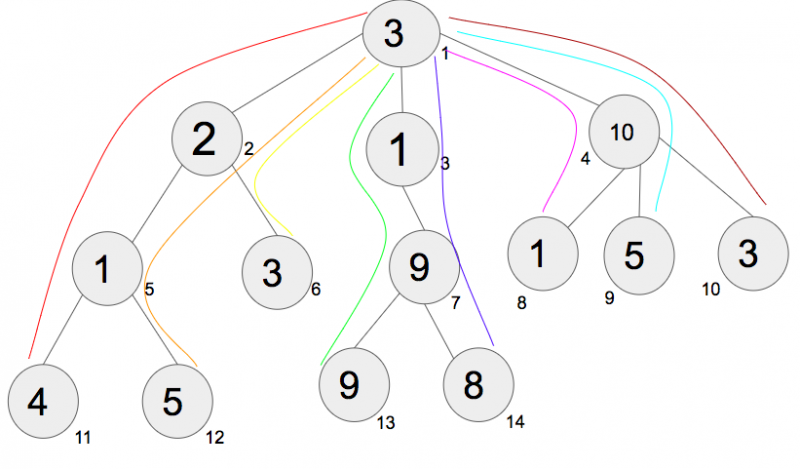
\includegraphics[width=0.3\textwidth]{Tree.png}
\end{center}

En el dibujo anterior, todos los caminos están marcados por diferentes colores, así:

\begin{itemize}[noitemsep]
\item Ruta 1(rojo, 3-2-1-4) : suma de todos los valores de los nodos = 10 
\item Ruta 2(naranja, 3-2-1-5) : suma de todos los valores de los nodos = 11 
\item Ruta 3(amarillo, 3-2-3) : suma de los valores de todos los nodos = 8 
\item Ruta 4(verde, 3-1-9-9) : suma de los valores de todos los nodos = 22 
\item Ruta 5(violeta, 3-1-9-8) : suma de los valores de todos los nodos = 21 
\item Ruta 6(rosa, 3-10-1) : suma de los valores de todos los nodos = 14 
\item Ruta 7(azul, 3-10-5) : suma de los valores de todos los nodos = 18 
\item Ruta 8(marrón, 3-10-3) : suma de los valores de todos los nodos = 16 
\end{itemize}

La respuesta para el árbol del dibujo es 22, ya que la ruta 4 tiene la máxima suma de valores de los nodos en su camino desde una raíz hasta las hojas. 

\hspace{1cm}

\textbf{Si trabajas en Java}, considera el siguiente código:

{\footnotesize
\begin{lstlisting}[language = java]
    static int[] dp = new int[100];
    // Realiza un recorrido en profundidad para guardar el valor maximo en dp[]
    private static void dfs(int[] a, Vector<Integer>[] v, int u, int parent){ 
        // Inicializamos dp[u] como a[u]
        dp[u] = a[u - 1];
        // Almacena el maximo valor de los nodos
        int maximum = 0;
        // Recorre el arbol
        for (int child : v[u]) {            
            // Si el hijo es padre, continuamos el ciclo
            if (child == parent)
                continue;
            // llamamos dfs para un recorrido nuevo
            dfs(a, v, child, u);            
            // Guarda el maximo entre un nodo previo y el nuevo visitado
            maximum = Math.max(maximum, dp[child]);
        }        
        // Agrega el maximo valor al nodo padre
        dp[u] += maximum;
    }
    // Funcion que retona el maximo valor de un arbol con nodo a y aristas v
    public static int maximumValue(int[] a, Vector<Integer>[] v) {
        dfs(a, v, 1, 0);
        return dp[1];
    }
\end{lstlisting}
}

  \begin{enumerate}[label=(\Alph*)]
    % O(V)
    \item (10\%) ¿Cuál es la complejidad asintótica, en el peor de los casos, del algoritmo anterior? Donde $V$ es el número de vértices del árbol.
    \begin{enumerate}[label=\roman*)]
      \item $O(V)$
      \item $O(V \times \log(V))$
      \item $O(V^2)$
      \item $O(1)$
      \item $O(V^3)$
      \item $O(\log(V))$
    \end{enumerate}
  \end{enumerate}



\newpage

\textbf{Si trabajas en Python}, considera el siguiente código:

\begin{lstlisting}
dp = [0]*100
# Realiza un recorrido en profundidad para guardar el valor maximo en dp[]
def dfs(a, v, u, parent):  
    #  Inicializamos dp[u] como a[u]
    dp[u] = a[u - 1]
    # Almacena el maximo valor de los nodos
    maximum = 0   
    # Recorre el arbol
    for child in v[u]:    
        # Si el hijo es padre, continuamos el ciclo
        if child == parent:
            continue        
        # llamamos dfs para un recorrido nuevo
        dfs(a, v, child, u)       
        # Guarda el maximo entre un nodo previo y el nuevo visitado
        maximum = max(maximum, dp[child])        
    # Agrega el maximo valor al nodo padre
    dp[u] += maximum
 
# Funcion que retona el maximo valor de un arbol con nodo a y aristas v
def maximumValue(a, v):
    dfs(a, v, 1, 0)
    return dp[1]
\end{lstlisting}

  \begin{enumerate}[label=(\Alph*)]
    % O(V)
    \item (10\%) ¿Cuál es la complejidad asintótica, en el peor de los casos, del algoritmo anterior? Donde $V$ es el número de vértices del árbol.
    \begin{enumerate}[label=\roman*)]
      \item $O(V)$
      \item $O(V \times \log(V))$
      \item $O(V^2)$
      \item $O(1)$
      \item $O(V^3)$
      \item $O(\log(V))$
    \end{enumerate}
  \end{enumerate}

\end{document}